\section{Systeme}
\subsection{Eigenschaften}
\begin{enumerate}
  \item{\textbf{Speicher}}\\
      % \begin{mdframed}[style=exercise]
          \bulletpt Frei: wird durch eine xy-Kennlinie vollständig
          beschrieben
          \[
              \text{z.B. \ }y(t)=\frac{R_1}{R_1+R_2}\cdot x(t)
          \]
          \bulletpt behaftet: Bei diesen Systemen ist keine
          vollständige Beschreibung durch eine xy-Kennline möglich
          \[
              \text{z.B. \ }y(t) = x(t)+2x(t-1)
          \]
      % \end{mdframed}
  \item{\textbf{Kausalit\"at}}\\
      % \begin{mdframed}[style=exercise]
           Ausgangssignal hängt nur vom aktuellen und vorherigen
           Eingangssignal ab
          \[
              \text{Kausal: z.B. \ }y(t) =
              \int\displaylimits_{t-5}^{t}x(\tau)d\tau
          \]
          \[
              \text{Akausal: z.B. \ }y(t) = x(t+1)-x(t-1)
          \]
      % \end{mdframed}

      \underline{Speicherfreiheit \& Kausalit\"at:} Aus Speicherfreiheit
      folgt Kausalität, aber nicht umgekehrt.
  \item{\textbf{Stabilit\"at}}\\
  (Bounded Input $\rightarrow$ Bounded Output)\\BIBO Stabilit\"at:
  kleines/beschr\"anktes Eingangssignal $\rightarrow$ kleine/beschr\"ankte
  Antwort.\\
  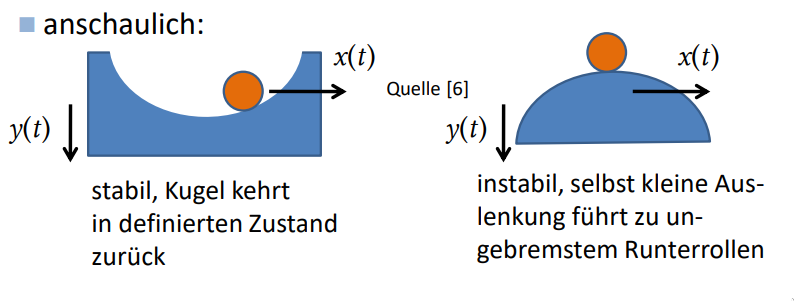
\includegraphics[width=.9\columnwidth]{Systeme/BIBO_anschaulich}\\
  % \begin{mdframed}[style=exercise]
      z.B. f\"ur stabiles System
  \[
      y(t) = 50\cdot x^3(t)
  \]\\
      z.B. f\"ur instabiles System
  \[
      y(t) = e^{t}\cdot x(t)
  \]
  % \end{mdframed}
  \item{\textbf{Zeitinvariant$\leftrightarrow$Zeitvariant}}\\
  \bulletpt invariant: Systeme \"andern sich \textbf{nicht} bei einer
  Zeitverschiebung.\\
  \bulletpt variant: Verschobenes Eingangssignal $\rightarrow$
  verschobenes Ausgangssignal
  \item{\textbf{Liniarit\"at}}\\
      Ein System ist linear, wenn das Superpositionsprinzip gilt:
      Linearkombination von Eingangssignalen ruft entsprechende
      Linearkombination der Ausgangssignale hervor
      \begin{mdframed}[style=exercise,frametitle=Bedeutung Liniarit\"at]
          eine Verdopplung der Eingangsgröße (z.B. Spannung) führt auch zu
          einer Verdopplung der Ausgangsgröße.
      \end{mdframed}
\end{enumerate}
\subsection{LTI-Systeme (Linear time-invariant Systems)}
\subsubsection{Ein-/Ausgangsbeziehung}
\begin{itemize}
  \item Addition
  \item Multiplikation
  \item Differentiation
  \item Integration
  \item Zeitverschiebung(Verz\"ogerung)
\end{itemize}
\subsubsection{Faltung}
Aus der Impulsantwort eines LTI-Systems und dem Eingangssignal lässt sich das
Ausgangssignal durch Faltung bestimmen:
\begin{mdframed}[style=exercise]
  \[
      y(t)=x(t)*h(t) \rightarrow (*)\text{ Faltung Operator}
  \]
  \[
      \boxed{y(t) = \int_{-\infty}^{+\infty} x(\tau)\cdot h(t-\tau)d\tau}
  \]
  \bulletpt Der Dirac-Impuls ist das neutrale Element der Faltung
  \[
      x(t)*\delta(t)=x(t)
  \]
  \bulletpt Eine Faltung mit einem verschobenen Dirac-Impuls führt zur Verschiebung
  des Signals:
  \[
      x(t)* \delta(t - a) = x(t - a)
  \]
\end{mdframed}
\begin{mdframed}[style=exercise,frametitle=Rechenregeln]
  \begin{itemize}
      \item{$x_1(t)*x_2(t)=x_2(t)*x_1(t)$}
      \item{$x_1(t)*[x_2(t)*x_3(t)]=[x_1(t)*x_2(t)]*x_3(t)$}
      \item{$x_1(t)*[x_2(t)+x_3(t)]=x_1(t)*x_2(t)+x_1(t)*x_3(t)$}
  \end{itemize}
\end{mdframed}
\subsection{Frequenzgang \& \"Ubertragungsfunktion}
\begin{mdframed}[style=exercise]
  \begin{itemize}
      \item{\textbf{Frequenzgang}}\\
          \[
              \underline{H}(\omega) =
              \frac{\underline{Y}(\omega)}{\underline{X}(\omega)} =
              \frac{\underline{U_2}(\omega)}{\underline{U_1}(\omega)}
          \]
      \item{\textbf{Amplitudengang}}\\
          \[
              A(\omega) = |\underline{H}(\omega)| =
              \frac{|\underline{Y}(\omega)|}{|\underline{X}(\omega)|}
              \begin{cases}
                  > 1 & \text{Verst\"arkung}\\
                  < 1 & \text{D\"ampfung}
              \end{cases}
          \]
      \item{\textbf{Phasengang}}\\
          \[
              \varphi_H(\omega) = \text{arg}\{\underline{H}(\omega)\} =
              \varphi_Y(\omega) - \varphi_X(\omega)
          \]
          \[
              \varphi_H = \text{arctan}(\frac{\mathfrak{Im}}{\mathfrak{Re}})
          \]
      \item{\textbf{Eigenfunktion}}\\
          \[
              y(t) = \lambda\cdot x(t)
              \begin{cases}
                  x(t): & \text{Eigenfunktion}\\
                  \lambda: & \text{Eigenwert}(\lambda\in\mathbb{C})
              \end{cases}
          \]
  \end{itemize}
\end{mdframed}
\begin{mdframed}[style=exercise]
  jede komplexe Exponentialfunktion $x(t) = \e^{st}$ ist Eigenfunktion
  jedes beliebigen LTI-Systems $S$:
  \[
      y(t) = S\left\{ \e^{st} \right\} = \lambda\cdot \e^{st}
  \]
  Eigenwert kann wie folgt berechnet werden:
  \[
      \lambda = \underline{H}(s) = \int_{-\infty}^{+\infty} h(\tau)\  \e^{-st} d\tau
  \]
  \begin{itemize}
      \item{\textbf{Erweiterung der komplexen Wechselstromrechnung}}\\
          Die harmonische Exponentialfunktion $e^{j\omega t}$ ist ein
          sonderfall von $e^{st}$ mit $s=j\omega$
          \[
              \sigma \triangleq Amplitude
              \begin{cases}
                  \sigma \leq 0 & \text{exponentiell abklingend}\\
                  \sigma = 0 & \text{konstante Amplitude}\\
                  \sigma \geq 0 & \text{exponentiell zunehmend}
              \end{cases}
          \]
          \[
              \omega \triangleq Rotation
              \begin{cases}
                  \omega \leq 0 & \text{Zeiger rotiert mit UZS}\\
                  \omega = 0 & \text{Zeiger rotiert nicht}\\
                  \omega \geq 0 & \text{Zeiger rotiert gegen UZS}
              \end{cases}
          \]
  \end{itemize}
\end{mdframed}
% \[
%   \boxed{
%   \begin{circuitikz}[scale=1,transform shape]
%       \draw(0,0) to[generic] node[anchor=east,yshift=-20pt]{$\underline{Z}(s)\mathrm{=}R$} (2,0);
%       \draw(3,0) to[L] node[anchor=east,yshift=-20pt, xshift=5pt]{$\underline{Z}(s)\mathrm{=}s\cdot L$} (5,0);
%       \draw(6,0) to[C, l=] node[anchor=east, yshift=-20pt, xshift=6pt]{$\underline{Z}(s)\mathrm{=}\frac{1}{s\cdot C}$} (8,0);
%   \end{circuitikz}
%   }
% \]

\begin{mdframed}[style=exercise,frametitle=Komplexe \"Ubertragungsfunktion]
  \footnotesize
  \[
      \underline{H}(s)=\frac{\underline{Y}(s)}{\underline{X}(s)}=\frac{\underline{U_2}(s)}{\underline{U_1}(s)}=\frac{\text{komplexer
      Zeiger des Ausgangssignals}}{\text{komplexer Zeiger des
      Eingangssignals}}
  \]
  \normalsize
  Die Übertragungsfunktion hängt von der komplexen\linebreak Frequenz
  \hl{$s=\sigma+j\omega$} ab.
\end{mdframed}
